\clearpage
\section{Long-Term Goal: Remote Neural Control}
\label{app:long-term}
This appendix preserves the generalized requirements, the original functional Figure 1, and the original high-workload Tables 1 and 2. They describe a research goal, not the installed robot or the first remote-control demonstration. A binary local I/O link, containerized neural simulator and 1\,kHz traffic are future choices; no replacement Pi model is specified. The current robot uses a Pi Model B Plus, a 2.4\,GHz USB Wi-Fi adapter and 115200-baud UART. Its existing local controller defaults to 20\,Hz; the implemented remote demonstration targets 100\,Hz and has been tested with motor output disabled.

The longer-term objective is line following through a remote spiking neural generator, including comparison of input-neuron selections and tolerable feedback delay. Live neurons remain an alternative source. A future forward-only wheel law is an experimental restriction; the current local controller permits reverse steering. The robot-motion model is retained separately in Appendix~\ref{sec:motion-control}.

\subsection{Future Functional Communication Schematic}
Figure~\ref{fig:functional-topology} preserves the original Figure 1 as a future concept; robot power distribution is in Section~\ref{sec:electrical-design}. The desktop's USB-C Ethernet adapter connects to an ASUS \emph{LAN} port. The current Pi uses a 2.4\,GHz USB Wi-Fi adapter; use that known connection as the initial transport baseline. In this future arrangement the desktop remains wired; only the last hop to the moving robot is wireless. The programming laptop reaches both computers through that same router, without requiring a second Pi radio. Router specifications are documented by \href{https://dlcdnets.asus.com/pub/ASUS/wireless/RT-N56U/E7822_RT_N56U_Manual_English.pdf}{ASUS}.

\begin{figure}[H]
\centering
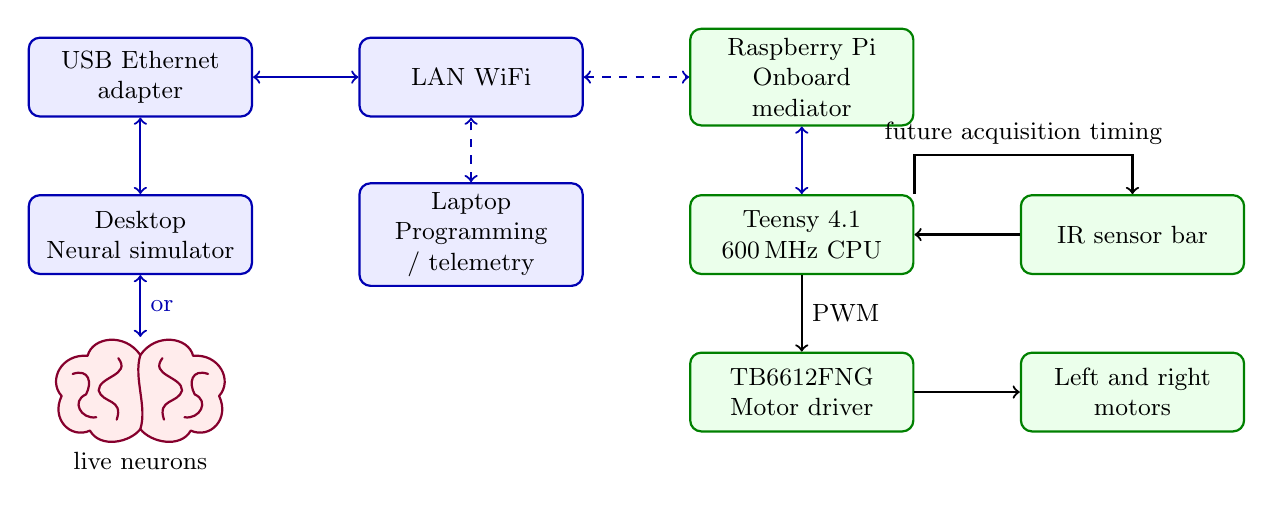
\begin{tikzpicture}[
    block/.style={draw=blue!70!black,fill=blue!8,rounded corners,thick,text width=2.6cm,align=center,minimum height=1.0cm,font=\small},
    hw/.style={block,draw=green!50!black,fill=green!8},
    wired/.style={<->,thick,blue!70!black},
    wireless/.style={wired,dashed}
]
\node[block] (adapter) at (0,4.0) {USB Ethernet\\adapter};
\node[block] (router) at (4.2,4.0) {LAN WiFi};
\node[hw] (pi) at (8.4,4.0) {Raspberry Pi\\Onboard mediator};
\node[block] (desktop) at (0,2.0) {Desktop\\Neural simulator};
\node[block] (laptop) at (4.2,2.0) {Laptop\\Programming / telemetry};
\node[hw] (teensy) at (8.4,2.0) {Teensy 4.1\\600\,MHz CPU};
\node[hw] (sensor) at (12.6,2.0) {IR sensor bar};
\node[hw] (driver) at (8.4,0) {TB6612FNG\\Motor driver};
\node[hw] (motor) at (12.6,0) {Left and right\\motors};
% Cartoon brain: an alternative neural source connected to the desktop.
\begin{scope}[draw=purple!70!black,line width=0.8pt,line cap=round,line join=round]
\path[draw,fill=pink!30]
    (0,0.47)
    .. controls (-0.20,0.76) and (-0.61,0.70) .. (-0.67,0.46)
    .. controls (-1.00,0.49) and (-1.18,0.15) .. (-1.00,-0.05)
    .. controls (-1.14,-0.34) and (-0.89,-0.60) .. (-0.64,-0.49)
    .. controls (-0.51,-0.72) and (-0.13,-0.64) .. (0,-0.47)
    .. controls (0.13,-0.64) and (0.51,-0.72) .. (0.64,-0.49)
    .. controls (0.89,-0.60) and (1.14,-0.34) .. (1.00,-0.05)
    .. controls (1.18,0.15) and (1.00,0.49) .. (0.67,0.46)
    .. controls (0.61,0.70) and (0.20,0.76) .. (0,0.47) -- cycle;
\draw (0,0.47) .. controls (-0.09,0.18) and (0.09,-0.18) .. (0,-0.47);
\foreach \side in {-1,1} {
    \begin{scope}[xscale=\side]
    \draw (0.28,0.43) .. controls (0.11,0.21) and (0.53,0.20) .. (0.53,0.02)
        .. controls (0.48,-0.15) and (0.21,-0.08) .. (0.30,-0.35);
    \draw (0.86,0.23) .. controls (0.65,0.30) and (0.61,0.12) .. (0.69,-0.03)
        .. controls (0.88,-0.11) and (0.76,-0.35) .. (0.56,-0.32);
    \end{scope}
}
\end{scope}
\node[font=\small] at (0,-0.88) {live neurons};
\draw[wired] (desktop.south) -- node[right,font=\small] {or} (0,0.70);
\draw[wired] (desktop) -- (adapter);
\draw[wired] (adapter) -- (router);
\draw[wireless] (router) -- (pi);
\draw[wireless] (laptop) -- (router);
\draw[wired] (pi) -- (teensy);
\draw[->,thick] (sensor) -- (teensy);
\draw[->,thick] (teensy.north east) -- ++(0,0.5) -| node[pos=0.25,above,font=\small] {future acquisition timing} (sensor.north);
\draw[->,thick] (teensy) -- node[right,font=\small] {PWM} (driver);
\draw[->,thick] (driver) -- (motor);
\end{tikzpicture}
\caption{Long-term functional layout (original Figure 1). The separate programming laptop and neural source are future elements, not the current deployment; the Pi model is left unspecified in this concept. Green boxes are on the robot platform. Solid links are wired; dashed links are wireless. Live neurons are shown as an alternative to the neural simulator, interfaced through the desktop. The programming laptop accesses the desktop and Pi through the ASUS router.}
\label{fig:functional-topology}
\end{figure}

\subsection{Future Workload and Connectivity Requirements}
Tables~\ref{tab:desktop-pi} and~\ref{tab:pi-teensy} preserve the original Tables 1 and 2 as future traffic sizing for the functional layout above. Rates use decimal kB/s. Payload bandwidth excludes framing, timestamps, sequence numbers, status, acknowledgements, overflow records, and transport overhead. The revised initial design uses 1\,kHz feedback, steering commands, and sensor reports; these controller rates are explicit configurable choices, distinct from the required 1\,ms neural step. A lower controller rate must be recorded with its command-hold policy and included in the delay experiment.

\begin{table}[H]
\centering\small
\caption{Desktop--Pi connectivity requirements and initial sizing}
\label{tab:desktop-pi}
\begin{tabular}{@{}L{3.0cm}L{6.2cm}L{7.3cm}@{}}
\toprule
\textbf{Item / direction} & \textbf{Required traffic or connection} & \textbf{Rate, capacity, or timing criterion} \\
\midrule
Desktop $\to$ Pi & One binary UDP datagram per native spike bin; 2-bit counts for every neuron & 1,000 frames/s; 50 B/frame at $N=200$: 50 kB/s; 125 B/frame at $N=500$: 125 kB/s \\
Pi $\to$ desktop & Selected-channel float32 requests; $m=20$ or 50 when selecting 10\% of neurons & Initially 1,000 commands/s; 80 or 200 B/command: 80 or 200 kB/s; generally $4m f_{\rm cmd}$ B/s \\
Combined payload & Both directions at the initial 1\,kHz rates & 130 kB/s (1.04 Mbit/s) baseline; 325 kB/s (2.60 Mbit/s) sizing case, plus overhead \\
Physical path & Desktop USB-C / USB 3 adapter $\to$ Gigabit Ethernet $\to$ ASUS RT-N56U LAN; router $\leftrightarrow$ Pi USB 2.4\,GHz radio (current baseline) & One wireless hop, a few metres; one Pi Wi-Fi adapter; router USB ports are not the desktop network connection \\
Delay and cadence & Preserve 1\,ms bin timestamps and transmit promptly; measure application-to-application age & Former USB references: 0.3--0.5 ms desktop-to-Pi equivalent and 0.2--0.3 ms return. These are comparison targets, not Wi-Fi guarantees; acceptance comes from the delay-margin experiment \\
Integrity and jitter & Sequence/bin IDs, command application acknowledgements, clock-offset/drift estimates or round-trip bounds & Report median, 99th/99.9th percentile and maximum observed delay, missing/late frames, longest interruption, and simulation deadline misses \\
\bottomrule
\end{tabular}
\end{table}

\begin{table}[H]
\centering\small
\caption{Pi--Teensy connectivity requirements and initial sizing}
\label{tab:pi-teensy}
\begin{tabular}{@{}L{3.0cm}L{6.2cm}L{7.3cm}@{}}
\toprule
\textbf{Item / direction} & \textbf{Required traffic or connection} & \textbf{Rate, capacity, or timing criterion} \\
\midrule
Pi $\to$ Teensy & Steering $u$ and baseline speed $v_0$; initial encoding: two float32 values & Initially 1,000 commands/s; 8 B payload: 8 kB/s. Add sequence, timestamp and validity information \\
Teensy $\to$ Pi & All three calibrated reflectances; proposed encoding: three float32 values & Initially 1,000 reports/s; 12 B payload: 12 kB/s. Add sample timestamp, sequence and status \\
Combined payload & Simultaneous command and sensor streams & 20 kB/s (0.160 Mbit/s), plus framing and status; this proposed 1\,kHz interface is separate from the current UART controller in Section~\ref{sec:local-controller} \\
Physical link & One onboard USB data cable; binary frames over USB CDC virtual serial & Bidirectional, asynchronous; The present Teensy uses external Vin with its USB power bridge cut; any future USB data link must preserve that power arrangement. Preserve frame boundaries in the application protocol \\
Transport and execution & Command delivery; timestamped sensor delivery; local command latch & Initial estimates: 0.2--0.3 ms Pi-to-Teensy and 0.3--0.5 ms return; verify experimentally. A chosen 1\,kHz latch adds up to one local tick after receipt \\
Validity and load & Bounded queues, stale-command timeout, sample IDs, configured stop/lost-link policy & No unbounded backlog; log missed reports and actual command age. Keep PWM and sensor acquisition independent of host delays \\
\bottomrule
\end{tabular}
\end{table}

\subsection{System Architecture \& Workload Segregation}
The closed loop has three compute nodes: the remote desktop, the onboard Pi, and the onboard Teensy. A separate programming laptop manages the desktop and Pi but does not participate in the timing-critical control loop.
\begin{itemize}
    \item \textbf{Remote neural simulation desktop:} A stationary macOS desktop running the controlled spiking SLDS in an Ubuntu 24.04 Podman container, with $N=200$ observed neurons ($N=500$ sizing case) and a 1\,ms step paced to wall-clock time. Use a native \texttt{linux/arm64} image on Apple Silicon. The desktop owns the generator state and applies timestamped feedback from the Pi.
    \item \textbf{Onboard mediator:} The Raspberry Pi receives spike packets, computes steering and selected-channel feedback, and retains optical sensor history. Benchmark the current Model B Plus before setting a sustainable workload; no future replacement model is selected. Its one radio carries both the neural traffic and management traffic.
    \item \textbf{Onboard real-time I/O:} One \href{https://www.pjrc.com/store/teensy41.html}{\textbf{Teensy 4.1}} (600\,MHz ARM Cortex-M7) manages local sensor acquisition, hardware timers and independent wheel PWM. The Pi connects to it over USB CDC.
    \item \textbf{Programming laptop:} A future separate service laptop can reach the simulator and Pi through ASUS. In the present setup, Desktop itself performs programming and management (Section~\ref{sec:network}). This service has no control-loop deadline and is intended for higher-throughput bulk transfers. Schedule large transfers outside trials; limit live telemetry during trials.
\end{itemize}

\subsection{Desktop Container and Shared-Network Operation}
On macOS, Podman runs Ubuntu containers inside a Linux virtual machine. macOS owns the USB Ethernet adapter; the container uses virtual networking, without USB passthrough. Publish the simulator's UDP feedback port, bind its receiver to all container interfaces, and send Pi feedback to the desktop's Ethernet IP address rather than its private container address. For example, publish \texttt{-p 0.0.0.0:5001:5001/udp}; the simulator sends spikes to the Pi's UDP port 5000. Use DHCP reservations or fixed addresses on one local subnet and verify inbound access through the desktop firewall. Podman's \texttt{--network=host} refers to the Linux VM, not directly to macOS. See the \href{https://docs.podman.io/en/latest/markdown/podman-machine-init.1.html}{Podman machine} and \href{https://docs.podman.io/en/latest/markdown/podman-run.1.html}{port-publishing documentation}.

Keep normal router mode with DHCP enabled for the standalone network and leave WAN unused; use the main LAN with client isolation disabled. For the current adapter choose a suitable 2.4\,GHz channel, disable Pi Wi-Fi power saving, and keep other connected networks on different subnets. The current baseline uses the 2.4\,GHz USB radio; management traffic still shares the final Wi-Fi hop. No internet connection is needed for the robot LAN. File transfers use reliable protocols such as SSH/SCP; live neural traffic uses binary UDP with explicit loss and lateness handling. A second Pi radio is unnecessary for this topology.

The desktop's simulator, VM scheduling, network queues, Wi-Fi contention and the Pi's processing all contribute delay and jitter. Sustaining 1,000 bins/s does not guarantee sub-millisecond delivery. Measure the full bidirectional workload while the robot moves and while bounded management telemetry is active. Keep simulator and Pi receive loops nonblocking, mark missing spike bins as missing rather than zero, and record deadline misses instead of hiding stalls with bursts of apparently current bins.

\subsection{Neural Model: Scope and Baseline}
\label{sec:controlled-neural}

\subsubsection{Objective, Dimensions, and Baseline}
The robot experiment evaluates \textbf{line-following control through spikes}; recovery of the hidden neural state is not an objective and no latent-state tracker is required in the control loop. The robot baseline uses $N=200$ observed neurons, latent dimension $d=5$, $K=3$ modes, and native step $\Delta=1\,\mathrm{ms}$. The communication sizing case retains $N=500$. Mode count and latent dimension are separate parameters: the three modes share a five-dimensional latent state.

The desktop simulator holds a fixed bank $\{A_s,\mu_s,Q_s\}_{s=0}^{K-1}$, the loading $C\in\mathbb{R}^{N\times d}$, calibrated baseline offsets $b_0\in\mathbb{R}^{N}$, and an uncontrolled transition matrix $\Pi^0$. Here $A_s$ is a \emph{discrete-time latent} matrix, not a synaptic connectivity matrix. Retain the baseline decay scale $\tau_A=10\,\mathrm{ms}$ and uncontrolled mean mode dwell $\tau_{\mathrm{dwell}}=300\,\mathrm{ms}$ as initial settings; both are swept in robot experiments. Fixed model coefficients do not imply stationary activity under sensor feedback. The zero-input generator is the stationary reference; the driven robot is a controlled switching system.

\subsubsection{Fixed Model Construction and Stationary Reference}
All times in equations are in seconds. The mode is $s_k\in\{0,\ldots,K-1\}$ and the latent state is $x_k\in\mathbb R^d$. A common uncontrolled mean dwell gives
\begin{equation}
 \Pi^0_{ii}=1-\frac{\Delta}{\tau_{\mathrm{dwell}}},\qquad
 \Pi^0_{ij}=\frac{\Delta}{(K-1)\tau_{\mathrm{dwell}}}\ (i\ne j),
 \qquad \pi^0_i=\frac1K.
 \label{eq:baseline-markov}
\end{equation}
Here $\pi^0$ is the stationary mode distribution. With $K=3$ and $\tau_{\mathrm{dwell}}=0.30$ s, the diagonal probability is $0.996\overline6$ and each off-diagonal probability is $0.001\overline6$. The latent state remains continuous across a mode change; it is not reset to the new center.

Construct the mode matrices in continuous time, then discretize:
\begin{equation}
 F_s=U\left(D_s+\frac{\nu}{\tau_A}J_s\right)U^{\top},\qquad
 A_s=\exp(F_s\Delta),\qquad U^{\top}U=I_d.
 \label{eq:bank-construction}
\end{equation}
The dimensionless parameter $\nu\ge0$ controls non-normal coupling. $D_s$ is real block diagonal with scalar blocks $-a/\tau_A$, $a>0$, or damped rotation blocks
\begin{equation}
 \frac1{\tau_A}\begin{pmatrix}-a&-\omega\\\omega&-a\end{pmatrix},
 \qquad a>0.
\end{equation}
$J_s$ is strictly block upper triangular in that partition, normalized to $\|J_s\|_F=1$. Its coupling changes transient behavior without changing the eigenvalues of the diagonal blocks. $U$ is a fixed shared orthogonal frame. Choose distinct centers $\mu_s\in\mathbb R^d$ and distinct mode matrices; save them rather than regenerating them during a run. One reproducible construction draws seeded Gaussian vectors $z_s$, sets $\bar z=K^{-1}\sum_s z_s$, and uses $\mu_s=\sigma_\mu(z_s-\bar z)$, with center scale $\sigma_\mu$ recorded. Similarly, a seeded Gaussian matrix followed by QR supplies $U$. The block coefficients, coupling matrices, and seed are configuration data.

For diffusion matrix $L\in\mathbb R^{d\times d}$, with units of latent state per square root second,
\begin{equation}
 Q_s=\int_0^\Delta e^{F_st}LL^{\top}e^{F_s^{\top}t}\,dt,
 \qquad \Sigma_s=A_s\Sigma_s A_s^{\top}+Q_s,\qquad
 \bar\Sigma=\frac1K\sum_s\Sigma_s.
 \label{eq:noise-lyapunov}
\end{equation}
A simple diffusion choice is $L=\sigma_L I_d$; $\sigma_L$ is saved with the bank. Compute exponentials, integrals, Lyapunov solutions, and a factor $Q_s=H_sH_s^{\top}$ offline on the desktop; share the accepted fixed model with the Pi. The desktop simulator generates $w_k=H_s\xi_k$, $\xi_k\sim\mathcal N(0,I_d)$. The fixed-mode covariance $\Sigma_s$ is not the conditional covariance of the switching process, which also contains transitions between centers.

Measure non-normality and transient gain over a declared horizon $H_{\mathrm{tr}}$ (initially $10\tau_A$):
\begin{equation}
 h_s=\frac{\|F_sF_s^{\top}-F_s^{\top}F_s\|_F}{\|F_s\|_F^2},\qquad
 G_s^{\mathrm{tr}}=\max_{0\le j\le\lfloor H_{\mathrm{tr}}/\Delta\rfloor}\|A_s^j\|_2.
 \label{eq:bank-transient}
\end{equation}
Require $\rho(A_s)<1$ in each mode and measured $G_s^{\mathrm{tr}}>1$ for a transient-amplifying bank. A $\nu=0$ bank is the normal-dynamics comparison. The time $\tau_A$ sets asymptotic decay: for a scalar decay block with $a=1$, a perturbation scales as $e^{-j\Delta/\tau_A}$. It does not set the mode dwell or guarantee an equally fast response in the presence of transient amplification.

For the uncontrolled switching linear part, form the $Kd^2\times Kd^2$ block operator
\begin{equation}
 \mathcal S^0_{ji}=\Pi^0_{ij}(A_j\otimes A_j),\qquad
 \rho(\mathcal S^0)<1.
 \label{eq:baseline-switch-stability}
\end{equation}
This tests mean-square stability of the zero-input bank; $\otimes$ denotes the Kronecker product and $\rho$ the spectral radius. The controlled bank must additionally satisfy the switching-stability requirement below. Record spectral margins, transient gains, and numerical acceptance thresholds with each accepted bank.

\subsubsection{Neural Loading, Rate Calibration, and Initialization}
Draw a fixed full-column-rank loading $C=\sigma_C\widehat C\in\mathbb R^{N\times d}$; for example, draw independent Gaussian rows and normalize each row of $\widehat C$ to unit Euclidean norm. Reject an ill-conditioned loading and record its singular values. Here $\sigma_C$ sets log-rate modulation depth. Define componentwise clipping by $\operatorname{clip}(z;l,h)=\min(h,\max(l,z))$; logarithms of rates use their numerical values in Hz.

Generate a discarded zero-input pilot of $T_p$ bins after burn-in, using the latent update in Equation~\eqref{eq:controlled-spikes} with all inputs zero. Write $b_{0,i}=\widehat b_i+\gamma$, where $\widehat b_i$ are fixed neuron offsets (zero is the simplest choice). For the pilot states $x_t^{(p)}$, choose the scalar $\gamma$ by monotone root finding so that
\begin{align}
 \bar f_i(\gamma)&=\frac1{T_p}\sum_{t=1}^{T_p}
  \exp\!\left[\operatorname{clip}(\widehat b_i+\gamma+C_{i:}x_t^{(p)};
       \log0.1,\log100)\right],\\
 \frac1N\sum_{i=1}^N\bar f_i(\gamma)&=8\ \mathrm{Hz}.
 \label{eq:pilot-rate}
\end{align}
This specifies a population mean target, useful for spike bandwidth estimates. Report $\operatorname{median}_i\bar f_i$ separately. Report both clamp fractions
\begin{equation}
 q_\pm=\frac1{NT_p}\sum_{t,i}
 \mathbf1\{\eta^{\mathrm{raw}}_{ti}\in\mathcal C_\pm\},\qquad
 \eta^{\mathrm{raw}}_{ti}=b_{0,i}+C_{i:}x_t^{(p)},\quad
 \eta_- =\log0.1,\quad\eta_+=\log100,
\end{equation}
where $\mathcal C_+=[\eta_+,\infty)$ and $\mathcal C_-=(-\infty,\eta_-]$, and $\mathbf1$ is the indicator function. If clamp occupancy exceeds the declared calibration limit, reduce loading or latent scales and recalibrate before evaluation. Freeze $C,b_0$ and all bank parameters after calibration.

Initialize the generator with $s_0\sim\operatorname{Categorical}(\pi^0)$ and $x_0\sim\mathcal N(\mu_{s_0},\Sigma_{s_0})$, then discard a separate zero-input burn-in. This initial Gaussian is a convenient seed, not an exact stationary switching-state draw. Start with a burn-in of $\max(20\tau_{\mathrm{dwell}},100\tau_A)$ and extend it if rate and latent moment checks have not stabilized. Save pilot length, burn-in length, initial state, and separate random seeds for model construction, calibration, and evaluation. Spikes are conditionally independent across neurons given the latent state and applied input; their shared fluctuations come from the latent dynamics. No synaptic connectivity or biological refractory period is represented.

\subsubsection{FFC and Projected-Transient Neuron Selection}
Use subspace dimension $r=2$ for $d=5$. Define the feed-forward controllable (FFC) proxy here as the dominant covariance frame:
\begin{equation}
 V_{\mathrm{FFC},s}=\operatorname{eig}_r(\Sigma_s),\qquad
 V_{\mathrm{FFC}}=\operatorname{eig}_r(\bar\Sigma),
 \label{eq:ffc-definition}
\end{equation}
where $\operatorname{eig}_r$ returns orthonormal eigenvectors for the $r$ largest eigenvalues. For each fixed mode, $\Sigma_s=\sum_{j\ge0}A_s^jQ_s(A_s^{\top})^j$ is the infinite-horizon noise-input Gramian. It need not equal the Gramian of the selected bias actuator $B_s$.

Define a comparison based on peak-transient directions:
\begin{align}
 j_s^\star&=\arg\max_{0\le j\le\lfloor H_{\mathrm{tr}}/\Delta\rfloor}\|A_s^j\|_2,
 &A_s^{j_s^\star}&=U_s^{\mathrm{tr}}S_s^{\mathrm{tr}}(V_s^{\mathrm{tr}})^{\top},\\
 Z_s&=(I_d-V_{\mathrm{FFC},s}V_{\mathrm{FFC},s}^{\top})U_{s,1:r}^{\mathrm{tr}},
 &P_s^{\mathrm{tr}}&=\operatorname{orth}(Z_s),\\
 \bar\Gamma^{\mathrm{tr}}&=\frac1K\sum_sP_s^{\mathrm{tr}}(P_s^{\mathrm{tr}})^{\top},
 &V_{\mathrm{tr}}&=\operatorname{eig}_r(\bar\Gamma^{\mathrm{tr}}).
 \label{eq:transient-selection}
\end{align}
Choose the earliest maximizing lag in a tie. If $Z_s$ has rank below $r$, use $P_s^{\mathrm{tr}}=U_{s,1:r}^{\mathrm{tr}}$ and flag the fallback. This projected-transient heuristic is not a proof of feedback controllability. Averaging projectors avoids the sign ambiguity of averaging basis vectors. The singular values $\sigma_\ell$ of $V_{\mathrm{FFC}}^{\top}V_{\mathrm{tr}}$ give principal angles $\theta_\ell=\arccos(\operatorname{clip}(\sigma_\ell;0,1))$; consensus frames need not be orthogonal.

For either frame $V_\bullet$, map to neurons and rank normalized row energies:
\begin{equation}
 W_\bullet=CV_\bullet,\qquad
 I_i^\bullet=\frac{\|W_\bullet(i,:)\|_2^2}
 {\max_j\|W_\bullet(j,:)\|_2^2},\qquad
 \mathcal I_\bullet=\operatorname{Top}_m(I_1^\bullet,\ldots,I_N^\bullet).
 \label{eq:neuron-ranking}
\end{equation}
Break score ties by neuron index. If every row energy is zero, reject that selection. Compare the top $m$ FFC neurons with the top $m$ transient neurons and report overlap. For mixed inputs, take $\lfloor m/2\rfloor$ top FFC neurons and fill the remaining slots with the highest-ranked unused transient neurons. Draw the random comparison uniformly without replacement using a saved seed. Keep $m$ identical across comparisons; exclusive top-score sets can be smaller and must not silently change the actuator budget.

\subsubsection{Selected Neurons and Explicit Input Authority}
The Pi knows the fixed model and selects an input subset $\mathcal I$ of size $m$ at initialization. Its selection matrix $S_{\mathcal I}\in\mathbb{R}^{N\times m}$ contains the corresponding columns of the identity. Start with $m=\mathrm{round}(0.10N)$, hence 20 channels at $N=200$, and keep $m$ configurable. FFC row-energy scores derived from $CV_{\mathrm{FFC}}$ provide the first selection rule. The steering decoder may use \textbf{all $N$ neurons}; input selection and output selection are independent.

The zero-input generator changes spike rates through $b_0+Cx$; emission bias alone does not actuate $x$ or the mode. The robot therefore adds two explicit control maps:
\begin{itemize}
\item $B_s\in\mathbb{R}^{d\times m}$: selected-channel input to the latent dynamics;
\item $R_i\in\mathbb{R}^{K\times m}$: selected-channel input to transition logits, conditional on source mode $i$.
\end{itemize}
These maps are part of the robot specification; they cannot be inferred as physical stimulation effects merely from knowing $A_s$ or the FFC frame. A reproducible initial synthetic choice is
\begin{equation}
 B_s=\beta_s C^{\top}S_{\mathcal I}/\zeta,\qquad
 \zeta=\max\{\|C^{\top}S_{\mathcal I}\|_2,\epsilon\},
 \label{eq:input-map}
\end{equation}
where $\epsilon>0$ is a saved numerical regularizer in the chosen latent units and $\beta_s$ sets latent displacement per native step per unit applied command. This back-projection is a declared modeling choice, not evidence of neuron-to-latent causality in the stationary generator. Precompute $B_s$ on the Pi; do not recompute it at every generator tick.

For a candidate input set, inspect the finite-horizon, fixed-mode input Gramian
\begin{equation}
 W_s(H)=\sum_{j=0}^{H-1} A_s^j B_sB_s^{\top}(A_s^{\top})^j,
 \label{eq:input-gramian}
\end{equation}
and the resulting signed steering response. Full latent controllability is not required for the scalar steering task, but the chosen input must have adequate authority in the decoded direction. FFC ranking alone is not a closed-loop performance guarantee. The projected peak-transient comparison defined below is a heuristic; its neuron scores do not establish input controllability.

\subsubsection{Bias Transport Delay and Neural Response Delay}
The Pi forms bounded selected-channel requests $a_k^{\mathrm{cmd}}\in\mathbb{R}^m$. Each message carries a sequence number and command timestamp. Model link/queue delay $D_k$ in native bins and a separate neural input time constant $\tau_b$:
\begin{align}
 a_k^{\mathrm{del}}&=a_{k-D_k}^{\mathrm{cmd}},\\
 \tilde a_k&=\alpha_b\tilde a_{k-1}+(1-\alpha_b)a_k^{\mathrm{del}},
 \qquad \alpha_b=e^{-\Delta/\tau_b},\\
 \delta b_k&=g_b S_{\mathcal I}\tilde a_k.
 \label{eq:bias-response}
\end{align}
Set $\alpha_b=0$ when $\tau_b=0$ and use zero input before the first command. The delay expression represents an ordered stream; a timestamped event queue implements variable latency, packet loss, and the configured stale-command policy without replaying obsolete commands. The desktop simulator latches inputs at a specified native-bin boundary and reports the sequence number and bin index when each request first enters its input filter. This acknowledgement distinguishes transport delay from slow neural response. Cross-device command ages require an estimated clock offset/drift or host round-trip timing bounds; raw timestamps from independent clocks are not directly subtracted.

The default $g_b=1$ preserves direct log-rate biasing of selected neurons. The same filtered command also enters the latent and mode equations below. Thus an input can affect rates directly, affect them through latent evolution, and alter future mode transitions. These routes must be tested separately: $g_b=0$ isolates dynamical effects; $B_s=R_i=0$ gives an emission-bias-only control. This prevents direct rate modulation from being mistaken for a benefit of non-normal dynamics.

\subsubsection{Controllable Markov Transitions}
Let $i=s_k$. Input modifies the next-mode transition row through bounded logits,
\begin{align}
 h_{ij,k}&=\log\Pi^0_{ij}
       +\operatorname{clip}\bigl((R_i\tilde a_k)_j;-\ell_{\max},\ell_{\max}\bigr),\\
 \bar\Pi_{ij,k}&=\frac{\exp(h_{ij,k}-\max_j h_{ij,k})}
                         {\sum_q\exp(h_{iq,k}-\max_j h_{ij,k})}.
 \label{eq:controlled-mode}
\end{align}
Use strictly positive $\Pi^0_{ij}$ for this baseline. Bound exit probability to avoid switching on nearly every 1-ms tick or effectively locking a mode:
\begin{align}
 p_{i,k}^{\mathrm{exit}}&=\operatorname{clip}
 \left(1-\bar\Pi_{ii,k};\Delta/\tau_{\max},\Delta/\tau_{\min}\right),\\
 \Pi_{ii,k}&=1-p_{i,k}^{\mathrm{exit}},\qquad
 \Pi_{ij,k}=p_{i,k}^{\mathrm{exit}}
       \frac{\bar\Pi_{ij,k}}{1-\bar\Pi_{ii,k}}\quad(j\ne i),\\
 s_{k+1}&\sim\operatorname{Categorical}(\Pi_{i:,k}).
 \label{eq:mode-exit}
\end{align}
Initial bounds are $\tau_{\min}=50\,\mathrm{ms}$ and $\tau_{\max}=3\,\mathrm{s}$; these bound the exit hazard, not the length of each realized dwell. At zero input the construction reproduces $\Pi^0$, whose 300-ms mean dwell lies inside these limits. Transitions remain stochastic: a command biases their probability, not their exact occurrence time.

One initial mode-targeting map is
\begin{equation}
 (R_i)_{j,:}=\kappa(\mu_j-\mu_i)^{\top}M B_i,
 \label{eq:mode-input-map}
\end{equation}
where $M=(\bar\Sigma+\epsilon I)^{-1}$ is a fixed positive-definite latent scaling matrix, $\bar\Sigma$ is the mean fixed-mode Lyapunov covariance, and $\kappa$ is a calibrated gain. This favors destinations aligned with the requested latent displacement. Verify that rows actually differ on the allowed inputs: adding an identical logit to every destination has no effect. The mode policy sees only the selected-channel command, not a hidden line-error shortcut. The actual mode is available locally to the desktop simulator; the Pi need not estimate or receive it for steering. Initial dimensionless limits are $a_{\max}=1$ and $\ell_{\max}=2$. Calibrate and store $\beta_s$, $\kappa$, the encoder $G$, and the decoder weights before evaluation; reject a bank/input map whose bounded commands cannot measurably alter destination probabilities and produce steering of both signs. Sweep $\tau_b$ from a zero-lag reference through 5, 10, 20, and 40 ms. For a mode-only ablation, retain the already calibrated $R_i$ when disabling $B_s$ in the latent update; do not recompute $R_i$ to zero.

\subsubsection{Latent Evolution and Spike Generation}
After the controlled mode draw, use
\begin{align}
 x_{k+1}&=\mu_{s_{k+1}}+A_{s_{k+1}}(x_k-\mu_{s_{k+1}})
          +B_{s_{k+1}}\tilde a_k+w_{k+1},\\
 w_{k+1}&\sim\mathcal N(0,Q_{s_{k+1}}),\\
 \eta_{k+1}&=\operatorname{clip}
   (b_0+Cx_{k+1}+\delta b_k;\log 0.1,\log100),\\
 \lambda_{k+1}&=\exp(\eta_{k+1}),\qquad
 n_{k+1,i}\sim\operatorname{Poisson}(\Delta\lambda_{k+1,i}).
 \label{eq:controlled-spikes}
\end{align}
This ordering defines the bin affected by an accepted request. All gains, input limits, initialization, random seeds, and timing parameters are saved with each trial. With zero input, this reduces to the stationary generator. Because the transition policy is now input dependent, the zero-input mean-square stability test in Equation~\eqref{eq:baseline-switch-stability} is insufficient. A conservative sufficient certificate is a common $P\succ0$ with $A_s^{\top}PA_s-P\prec0$ for every mode; bounded inputs and mode centers then act as bounded forcing with finite process-noise covariance. Failure to find a common certificate is not itself proof of instability, but requires a more specific controlled-switching analysis and stress testing.

The baseline population mean-rate target is 8 Hz/neuron, calibrated by Equation~\eqref{eq:pilot-rate}. Also record the median across neuron mean rates; it need not equal the population mean. Keep the 100-Hz upper clamp initially. A neuron at 8 Hz reaches 100 Hz after an unclipped log-rate increase of $\log(100/8)\simeq2.53$, which can arise from mode centers, non-normal transients, or input. Whether this occurs must be measured, not inferred from the baseline rate alone. Report unclipped log-rate quantiles, per-neuron clamp occupancy, and command-conditioned saturation. Do not raise the clamp merely to obtain more steering authority. A Poisson rate cap bounds the conditional intensity, not the number of spikes in an individual bin, and does not impose a biological refractory period. A refractory generator would be a separate, recalibrated variant.

\subsubsection{Pi Readout, Sensor History, and Forward Steering}
The Pi retains timestamped histories of the three calibrated reflectances, estimated line position, confidence, spike packets, and previous commands. The initial selected-channel encoder is a bounded causal map of line-error history, for example
\begin{equation}
 a_k^{\mathrm{cmd}}=\operatorname{clip}
    \left(G\phi_k;-a_{\max},a_{\max}\right),\qquad
 \phi_k=[e_k,\dot e_k^{\mathrm{filtered}},\ldots]^{\top},
 \label{eq:sensor-encoder}
\end{equation}
with confidence gating and a declared lost-line policy. Teensy samples sensors and reports them to the Pi; it does not need to reconstruct the neural state. This placement gives the Pi ownership of sensor history and of the bias requests sent to the desktop simulator.

The motor decoder uses all neurons if desired. For causal filtered rates,
\begin{equation}
 r_k=\alpha_r r_{k-1}+(1-\alpha_r)n_k/\Delta,\qquad
 \alpha_r=e^{-\Delta/\tau_r},\qquad
 u_k=\tanh\bigl(w^{\top}(r_k-r_0)+c\bigr).
 \label{eq:steering-readout}
\end{equation}
No $\hat x_k$ or inferred mode is needed. Calibrate $w,r_0,c$ so a centered line gives near-zero mean steering across modes, and measure the remaining variance and switch-triggered excursions. Use generator truth only for offline diagnosis and evaluation; a decoder supplied with true mode labels is an explicitly labelled oracle ablation, not the operational controller.

Use $u\in[-1,1]$ for steering, reserving $x$ for the latent state. For $u>0$ (right turn), slow the right wheel; for $u<0$ (left turn), slow the left wheel:
\begin{equation}
 v_L^{*}=v_0\bigl(1-\max(0,-u)\bigr),\qquad
 v_R^{*}=v_0\bigl(1-\max(0,u)\bigr).
 \label{eq:forward-wheel-law}
\end{equation}
At $u=0$ both targets equal $v_0$; at $|u|=1$ the inner wheel stops. Neither reverses. If both must remain strictly moving, impose $|u|\le u_{\max}<1$. For wheel separation $L_w$, the ideal mean speed is $v_0(1-|u|/2)$ and clockwise yaw rate is $v_0u/L_w$. At full steering the minimum ideal axle-centre turn radius is $L_w/2$; forward-only steering cannot turn about the axle centre.

Teensy has two independent wheel command channels. With no encoders, the physical implementation is calibrated PWM and cannot verify actual speed; an ideal speed actuator is only the first simulation condition. Add unequal gains, lag, deadband, battery/load effects, and slip to subsequent trials. Later encoders can close independent local wheel-speed loops, and absolute motion tracking can supply evaluation ground truth without changing the neural steering interface.

\subsection{Delay-Margin Experiment and Comparisons}
The main experiment estimates the \textbf{largest tolerable feedback delay} for a declared speed, track family, neural model, and success criterion. There is no single universal delay limit. Sweep added command delay initially over 0, 2, 5, 10, 20, 40, 80, and 160 ms, refine around failures, and repeat across seeds; separately sweep $\tau_b$, rate-filter time $\tau_r$, and timing jitter. Zero added delay still retains the sampled update ordering and any modeled actuator response. Link latency, input filtering, latent response, random mode-switch waiting time, stochastic first-spike waiting time, readout filtering, and wheel lag are distinct contributions. Do not interpret the first observed post-command spike as a deterministic latency measurement: compare repeated paired trials with matched seeds and measure changes in expected rates and steering as well as first-spike statistics.

For each setting, report RMS and high-percentile line error, line-loss probability, completed distance/laps, steering variation, clamp occupancy, and actual command age. Define success thresholds before the sweep and report success probability across seeds rather than assuming a monotone binary delay boundary. Start with ideal forward wheel dynamics, then repeat with motor mismatch and jitter. Include the following matched comparisons:
\begin{itemize}
\item FFC-selected, random, mixed, and projected-transient-selected input neurons as defined above, with the same input count, bias limits, comparable delivered input energy and firing-rate budget, and normalized latent/mode gains;
\item all-neuron versus sparse spike readouts, each calibrated with the same training budget;
\item emission-only, latent-only, mode-only, and combined input routes;
\item stochastic spikes versus conditional expected rates, and a conventional sensor controller as a performance reference.
\end{itemize}
For meaningful input-subset comparisons, keep the underlying neuron-to-latent and neuron-to-logit mapping rule fixed and select its columns; do not give each subset an independently optimized arbitrary actuator. No conventional controller contributes hidden corrective steering during evaluation of the neural loop. A one-mode run can diagnose dynamics and transport, but the primary robot experiment retains the configurable three-mode model.

\subsection{Real-Time Control Protocol \& Closed-Loop Data Pipeline}
The asynchronous loop is desktop spike generation $\to$ Pi readout $\to$ Teensy wheel commands and sensor acquisition $\to$ Pi sensor-history encoder $\to$ desktop neural feedback. The desktop--Pi link uses UDP over wired Ethernet plus one Wi-Fi hop; the Pi--Teensy link uses USB CDC. Tables~\ref{tab:desktop-pi} and~\ref{tab:pi-teensy} give the traffic requirements. Neither link is a blocking request--response chain.

\subsubsection{Data Payloads \& Packing}
Use packed binary frames with an explicitly defined byte order, frame type, length, sequence and timestamp/bin fields. USB CDC is a byte stream, so handle partial reads and multiple frames per read. UDP preserves datagram boundaries, but the receiver must detect missing, duplicate, reordered and late packets. UDP does not remove Wi-Fi's own link-layer retries. Keep application queues bounded and log all drops; declare the missing-bin decoder policy and stale-command policy with each trial.
\begin{itemize}
    \item \textbf{Desktop $\to$ Pi (spikes):} One native bin per UDP datagram at 1\,kHz. The default 2-bit format encodes counts 0--3 and uses 50 bytes for 200 neurons or 125 bytes for 500. Framing and a clipping indicator/counter are additional; counts above 3 are logged and optionally sent as overflow records. A 1-bit occupancy ablation uses 25 or 63 bytes, respectively. Send each bin promptly; batching ten bins adds up to 9\,ms of waiting to the oldest bin.
    \item \textbf{Pi $\to$ Teensy (actuation):} Initially two float32 values, steering $u$ and speed $v_0$, plus sequence, timestamp and validity information. Teensy applies Equation~\eqref{eq:forward-wheel-law} independently to the wheels, with a local stale-command timeout and configured stop policy.
    \item \textbf{Teensy $\to$ Pi (sensors):} Proposed: three float32 calibrated reflectances, plus acquisition timestamp, sequence and status. The Pi retains sensor history and computes line-error features.
    \item \textbf{Pi $\to$ desktop (neural feedback):} Timestamped selected-channel requests $a^{\mathrm{cmd}}$ or compact encoder coefficients. A float32 vector is 80 bytes for $m=20$ and 200 bytes for $m=50$. Configure fixed maps and neuron indices once; compact coefficients are valid only if the desktop expands the same configured map. Each accepted request is acknowledged with its sequence and effective generator bin. Between accepted commands, hold the latest valid request before the neural input filter, subject to the configured expiry policy.
\end{itemize}

For a constant per-neuron rate $f$, put $\mu=f\Delta$. The probability of multiplicity is $p_{\ge2}=1-e^{-\mu}(1+\mu)$; converting counts to occupancy loses the fraction $1-(1-e^{-\mu})/\mu$ of expected spikes. At 8 Hz and 1 ms these are approximately 0.00318\% of bins and 0.399\% of spikes; at 100 Hz they are 0.468\% and 4.84\%, respectively. Thus 1-bit packing is a reasonable measured approximation near baseline, but 2-bit counts cheaply preserve most multiplicity at higher transient rates. Two bits encode 0--3, three encode 0--7, and four encode 0--15: an inclusive clip value of 4 needs three bits, and 8 needs four. Preserve full counts in the reference simulator and compare each wire-format approximation with it. At 100 Hz, the probability of a count exceeding 3 is about $3.85\times10^{-6}$ per bin, small but not zero. Record overflow rather than silently treating the clipped distribution as exact Poisson data.

\subsubsection{Closed-Loop Timing Budget and Validation}
The former all-USB estimate of approximately 12.0--12.7\,ms is not a prediction for the revised wireless/container system. Measure the terms below under the actual bidirectional workload. The original 5\,ms Pi compute entries cannot describe serial processing of every incoming 1\,ms frame: that would accumulate a backlog. With the initial 1\,kHz controller, benchmark the combined Pi readout/encoder workload for sustained service within the available 1\,ms cycle, or explicitly choose and report a slower controller schedule while still consuming every neural bin.

\begin{table}[H]
\centering\small
\caption{Timing terms for the remote-desktop loop; values marked as references are not guarantees}
\label{tab:timing_budget}
\begin{tabular}{@{}L{3.2cm}L{8.2cm}L{5.1cm}@{}}
\toprule
\textbf{Term} & \textbf{Measurement boundary / requirement} & \textbf{Initial reference or acceptance basis} \\
\midrule
Spike delivery & Desktop bin ready to Pi application receive; includes container/VM, Ethernet and Wi-Fi & Measure distribution; former USB reference 0.3--0.5 ms \\
Pi readout & Receive/decode/filter spikes and generate wheel request & Benchmark actual service time and scheduling delay; sustain 1,000 bins/s \\
Wheel command delivery & Pi application send to Teensy complete-frame receipt & USB reference 0.2--0.3 ms; measure \\
Local I/O & Command receipt to local latch; timestamp actual optical acquisition separately & Initial 1\,kHz I/O schedule; up to one tick of latch wait, plus execution \\
Sensor delivery & Timestamped sensor frame ready on Teensy to Pi application receive & USB reference 0.3--0.5 ms; measure \\
Pi feedback compute & Sensor history update and selected-channel encoding & Benchmark jointly with readout; initial feedback period 1 ms \\
Feedback delivery & Pi send to desktop simulator receive, including VM ingress & Measure distribution; former USB reference 0.2--0.3 ms \\
Generator acceptance & Desktop receipt to request entering input filter at a native-bin boundary & Up to one 1\,ms bin under on-time scheduling; record VM/simulator deadline misses \\
\bottomrule
\end{tabular}
\end{table}

Assemble latency from measured causal intervals, including scheduling waits; its inverse is not the controller frequency. Align the VM, Pi and Teensy clock domains, or report round-trip bounds. Input filtering, latent/mode response, readout filtering and motor lag remain separate contributions to the delay-margin experiment in Section~\ref{sec:controlled-neural}.

Validate both neuron counts with simultaneous bidirectional traffic, robot motion and bounded management telemetry. Report the packet-age/loss metrics in Table~\ref{tab:desktop-pi}, queue depths and actual command application ages. Judge the measured delay/jitter profile against the declared line-following success criteria. Neither 1\,kHz cadence nor adequate average bandwidth establishes a hard deadline; Wi-Fi and macOS/VM scheduling provide no hard sub-millisecond guarantee.

